\title{CS 383 - Machine Learning}
\author{
Assignment 1 - Dimensionality Reduction\\
Summer 2017\\
Amir Omidi
}
\date{}
\documentclass[12pt]{article}
\usepackage[margin=0.7in]{geometry}
\usepackage{graphicx}
\usepackage{float}
\usepackage{amsmath}


\begin{document}
\maketitle

\newpage
\section{Theory Questions}
\subsection{Question 1}
\subsubsection{Part A}
\noindent

Our starting data for this section is the following:

\begin{center}
$\begin{bmatrix}
-2 & 1\\
-5 & -4\\
-3 & 1\\
0 & 3\\
-8 & 11\\
-2 & 5\\
1 & 0\\
5 & -1\\
-1 & -3\\
6 & 1\\
\end{bmatrix}$
\end{center}


\noindent
We need to standardize our data before we get started with PCA. To do this we need the average and standard deviation of each column.\\


\noindent
Lets first calculate the average of each column:\\
\begin{itemize}
\item
Column 1 average:\\

\begin{center}
$\frac{-2-5-3+0-8-2+1+5-1+6}{10} = -0.9$\\
\end{center}

\item
Column 2 average:\\

\begin{center}
$\frac{1-4+1+3-11+5+0-1-3+1}{10} = 1.4$\\
\end{center}

\end{itemize}


\noindent
Now we should calculate the standard deviation of each column using the average we calculated above.\\
\begin{itemize}
\item
Column 1 standard deviation:\\

\begin{itemize}
\item
Find variance squared of each row:\\

\begin{enumerate}
\item
$ (-2+0.9)^2 = 1.21$
\item
$ (-5+0.9)^2 = 16.81$
\item
$ (-3+0.9)^2 = 4.41$
\item
\ldots
\end{enumerate}

\item
Add them all up:\\
\begin{center}
$1.21+16.81+4.41+0.81+50.41+1.21+3.61+34.81+0.01+47.61 = 160.90$
\end{center}

\item
Since we're calculating a sample standard deviation, we divide the sum by 9 ($sample size - 1$) and then take a square root of it.\\
\begin{center}
$\sqrt{\frac{160.90}{9}} = 4.2282$
\end{center}

\end{itemize}

\item
Column 2 standard deviation:\\

\begin{itemize}
\item
Find variance squared of each row:\\

\begin{enumerate}
\item
$ (1-1.4)^2 = 0.16$
\item
$ (-4-1.4)^2 = 29.16$
\item
$ (1-1.4)^2 = 0.16$
\item
\ldots
\end{enumerate}

\item
Add them all up:\\
\begin{center}
$0.16+29.16+0.16+2.56+92.16+12.96+1.96+5.76+19.36+0.16 = 164.40$
\end{center}

\item
Since we're calculating a sample standard deviation, we divide the sum by 9 ($sample size - 1$) and then take a square root of it.\\
\begin{center}
$\sqrt{\frac{160.40}{9}} = 4.27395$
\end{center}

\end{itemize}
\end{itemize}
\noindent
Now we can start standardizing our matrix.
\begin{itemize}
\item
Standardization 1 - We can now begin standardizing our data. The first step is to subtract the mean of each column from the elements of each column:\\
\begin{center}
$\begin{bmatrix}
-1.1 & -0.4\\
-4.1 & -5.4\\
-2.1 & -0.4\\
0.9 & 1.6\\
-7.1 & 9.6\\
-1.1 & 3.6\\
1.9 & -1.4\\
5.9 & -2.4\\
-0.1 & -4.4\\
6.9 & -0.4\\
\end{bmatrix}$
\end{center}

\item
Standardization 2 - The second step is to divide each element of each column by the standard deviation of that column:\\
\begin{center}
$\begin{bmatrix}
-0.2602 & -0.0936\\
-0.9697 & -1.2635\\
-0.4967 & -0.0936\\
0.2129 & 0.3744\\
-1.6792 & 2.2462\\
-0.2602 & 0.8423\\
0.4494 & -0.3276\\
1.3954 & -0.5615\\
-0.0237 & -1.0295\\
1.6319 & -0.0936\\
\end{bmatrix}$
\end{center}
\end{itemize}

\noindent
The next step is to calculate the covariance of the matrix.

We will be using the following formula: $X'X/(N-1)$

\begin{center}
$
\begin{bmatrix}
-0.2602 & -0.9697 & -0.4967 & 0.2129 & -1.6792 & -0.2602 & 0.4494 & 1.3954 & -0.0237 & 1.6319\\

-0.0936 & -1.2635 & -0.0936 & 0.3744 & 2.2462 & 0.8423 & -0.3276 & -0.5615 & -1.0295 & -0.0936\\
\end{bmatrix}
\times
\begin{bmatrix}
-0.2602 & -0.0936\\
-0.9697 & -1.2635\\
-0.4967 & -0.0936\\
0.2129 & 0.3744\\
-1.6792 & 2.2462\\
-0.2602 & 0.8423\\
0.4494 & -0.3276\\
1.3954 & -0.5615\\
-0.0237 & -1.0295\\
1.6319 & -0.0936\\
\end{bmatrix}
\times
\frac{1}{9}
=
\begin{bmatrix}
1.0000 & -0.4083 \\
-0.4083 & 1.0000 \\
\end{bmatrix}
$

\end{center}

\noindent
Now that we have the covariance matrix, finding the eigenvalues is an easy task.

\begin{center}
$
\begin{bmatrix}
1 - \lambda & -0.4083\\
-0.4083 & 1 - \lambda \\
\end{bmatrix}
\Rightarrow
\lambda^2 - 2\lambda+(1-(-0.4083)^2)=\lambda^2+2\lambda+0.8333
$
\\
$
\lambda=0.5917, 1.4083
$
\end{center}

\noindent
Now that we have the eigenvalues, we need to find the eigenvectors.
\begin{center}

$
\begin{bmatrix}
1.0000 & -0.4083 \\
-0.4083 & 1.0000 \\
\end{bmatrix}
-
\begin{bmatrix}
0.5917 & 0 \\
0 & 0.5917 \\
\end{bmatrix}
=
\begin{bmatrix}
0.4083 & -0.4083 \\
-0.4083 & 0.4083 \\
\end{bmatrix}
$
\\[0.1 in]
$
\begin{bmatrix}
0.4083 & -0.4083 \\
-0.4083 & 0.4083 \\
\end{bmatrix}
\times
\begin{bmatrix}
a \\
b \\
\end{bmatrix}
=
\begin{bmatrix}
0 \\
0 \\
\end{bmatrix}
$
\\[0.1 in]
$
\begin{matrix}
0.4083a - 0.4083b = 0\\
-0.4083a + 0.4083b = 0 \\
\end{matrix}
\Rightarrow b=t
$
\\[0.1 in]
\end{center}
Eigenvector is any scalar multiple of
$
\begin{bmatrix}
1 & 1
\end{bmatrix}
^T
$
\\[0.1 in]
And for the other eigenvalue, doing the above steps we see that it is any scalar multiple of:
$
\begin{bmatrix}
-1 & 1
\end{bmatrix}
^T
$
\par

\subsubsection{Part B}
The largest eigenvalue is clearly 1.4083. The corresponding eigenvector for that eigenvalue is mentioned above. By multiplying the data with that eigenvector we would successfully project the data onto the PCA of the largest eigenvalue and reduced the conventionality of the data from $D=2$ to $D=1$.
\begin{center}

$\begin{bmatrix}
-0.2602 & -0.0936\\
-0.9697 & -1.2635\\
-0.4967 & -0.0936\\
0.2129 & 0.3744\\
-1.6792 & 2.2462\\
-0.2602 & 0.8423\\
0.4494 & -0.3276\\
1.3954 & -0.5615\\
-0.0237 & -1.0295\\
1.6319 & -0.0936\\
\end{bmatrix}
\times
\begin{bmatrix}
-1 \\
1
\end{bmatrix}
=
\begin{bmatrix}
0.1667\\
-0.2938\\
0.4031\\
0.1615\\
3.9254\\
1.1025\\
-0.7769\\
-1.9569\\
-1.0058\\
-1.7255\\
\end{bmatrix}
$

\end{center}

\subsection{Question 2}
\subsubsection{Part A}

We have two classes of data:
\begin{center}
$
Positive =
\begin{bmatrix}
-2 & 1\\
-5 & -4\\
-3 & 1\\
0 & 3\\
-8 & 11\\
\end{bmatrix}
, Negative =
\begin{bmatrix}
-2 & 5\\
1 & 0\\
5 & -1\\
-1 & -3\\
6 & 1\\
\end{bmatrix}
$
\\[0.1 in]
\end{center}

These are the labels that we have:
\begin{center}
$
Labels\in\{-8, -5,-4,-3,-2,-1,0,1,3,5,6,11\}
$
\\[0.1 in]
\end{center}
\noindent
Let's start with the process of information gain.

\noindent
\textbf{Feature one}
\begin{center}

\begin{align*}
&p_{-8}=1, &n_{-8}=0\\
&p_{-5}=1, &n_{-5}=0\\
&p_{-4}=0, &n_{-4}=0\\
&p_{-3}=1, &n_{-3}=0\\
&p_{-2}=1, &n_{-2}=1\\
&p_{-1}=0, &n_{-1}=1\\
&p_{0}=1, &n_{0}=0\\
&p_{1}=0, &n_{1}=1\\
&p_{3}=0, &n_{3}=0\\
&p_{5}=0, &n_{5}=1\\
&p_{6}=0, &n_{6}=1\\
&p_{11}=0, &n_{11}=0\\
\end{align*}
\\[0.1 in]
\end{center}

\noindent

Now we plug them into the remainder formula:

\begin{center}

\begin{align*}
Reamainder(1) =\\
&\frac{1}{10} \times [(\frac{-1}{1}\log_{2}{\frac{1}{1}}) + 0] &&\text{This is 0}\\
+ &0 &&\text{This is for label -5 which is also 0.} \\
+ &0 &&\text{Same as above.}\\
+ &0\\
+ &\frac{2}{10} \times [(\frac{-1}{2}\log_{2}{\frac{1}{2}}) + (\frac{-1}{2}\log_{2}{\frac{1}{2}})] &&\text{This is } \frac{1}{5}\\
+ &0\\
+ &0\\
+ &0 \\
+ &\ldots\\
&=  \frac{1}{5}
\end{align*}

\begin{align*}
Remainder(1) = \frac{1}{5} = 0.2000
\end{align*}
\\[0.1 in]
\end{center}

\noindent
\textbf{Feature two}
\begin{center}


\begin{align*}
&p_{-8}=0, &n_{-8}=0\\
&p_{-5}=0, &n_{-5}=0\\
&p_{-4}=1, &n_{-4}=0\\
&p_{-3}=0, &n_{-3}=1\\
&p_{-2}=0, &n_{-2}=0\\
&p_{-1}=0 ,&n_{-1}=1\\
&p_{0}=0, &n_{0}=1\\
&p_{1}=2, &n_{1}=1\\
&p_{3}=1, &n_{3}=0\\
&p_{5}=0, &n_{5}=1\\
&p_{6}=0, &n_{6}=0\\
&p_{11}=1, &n_{11}=0\\
\end{align*}
\\[0.1 in]
\end{center}

\noindent

Now we plug them into the remainder formula:

\begin{center}

\begin{align*}
Reamainder(2) =\\
&\frac{3}{10} \times [(\frac{-2}{3}\log_{2}{\frac{2}{3}}) + (\frac{-1}{3}\log_{2}{\frac{1}{3}})]
&= 0.2755
\end{align*}

\begin{align*}
Remainder(2) = 0.275
\end{align*}
\\[0.1 in]
\end{center}
\textbf{The information gain for each feature}
\begin{center}

\begin{align}
IG(1) = [2 \times (\frac{-5}{10}\log_{2}{\frac{5}{10}})] - 0.2000 = 0.8000 \\
IG(2) = [2 \times (\frac{-5}{10}\log_{2}{\frac{5}{10}})] - 0.2755 = 0.7245
\end{align}
\\[0.1 in]
\end{center}

\noindent
\subsubsection{Part B}

As you can clearly see from equations 1 and 2, the more discriminating feature is feature 1.

\noindent
\subsubsection{Part C}
Let's start by standardizing our entire data set. The standardized matrix was already found in Question 1 part a.

\begin{center}
$
standardize(
\begin{bmatrix}
-2 & 1\\
-5 & -4\\
-3 & 1\\
0 & 3\\
-8 & 11\\
-2 & 5\\
1 & 0\\
5 & -1\\
-1 & -3\\
6 & 1\\
\end{bmatrix}
)=\begin{bmatrix}
-0.2602 & -0.0936\\
-0.9697 & -1.2635\\
-0.4967 & -0.0936\\
0.2129 & 0.3744\\
-1.6792 & 2.2462\\
-0.2602 & 0.8423\\
0.4494 & -0.3276\\
1.3954 & -0.5615\\
-0.0237 & -1.0295\\
1.6319 & -0.0936\\
\end{bmatrix}
$
\\[0.1 in]
\end{center}
We should get the mean of each class now:
\begin{center}
\begin{align}
&\mu_{1} = mean\left(\begin{bmatrix}
-0.2602 & -0.0936\\
-0.9697 & -1.2635\\
-0.4967 & -0.0936\\
0.2129 & 0.3744\\
-1.6792 & 2.2462\\
\end{bmatrix}\right)
=
\begin{bmatrix}
-0.6386 & 0.2340\\
\end{bmatrix} \label{mean1} \\
&\mu_{2} = mean\left(\begin{bmatrix}
-0.2602 & 0.8423\\
0.4494 & -0.3276\\
1.3954 & -0.5615\\
-0.0237 & -1.0295\\
1.6319 & -0.0936\\
\end{bmatrix}\right)
=
\begin{bmatrix}
0.6386 & -0.2300
\end{bmatrix}\label{mean2}
\end{align}
\end{center}

We can use this data to calculate $S_{B}$:
\begin{center}
\begin{gather}
\mu_{1} - \mu_2 =
\begin{bmatrix}
-1.2771 & 0.4680\\
\end{bmatrix} \nonumber \\
S_{B} = \begin{bmatrix}
-1.2771\\
0.4680\\
\end{bmatrix}
\times
\begin{bmatrix}
-1.2771 & 0.4680\\
\end{bmatrix}
=
\begin{bmatrix}
1.6311 && -0.5976\\
-0.5976 && 0.2190\\
\end{bmatrix}
\end{gather}
\end{center}
Now, we need to calculate the scatter matrices for each class. Before we do that, we need to calculate the covariance matrix for each class. In order to do this, we need to standardize each class to be able to find the covariance easier.

\begin{center}
$
\begin{bmatrix}
-2 & 1\\
-5 & -4\\
-3 & 1\\
0 & 3\\
-8 & 11\\
\end{bmatrix}
-
\left(
\begin{bmatrix}
1 & 1 & 1 & 1 & 1\\
1 & 1 & 1 & 1 & 1\\
1 & 1 & 1 & 1 & 1\\
1 & 1 & 1 & 1 & 1\\
1 & 1 & 1 & 1 & 1\\
\end{bmatrix}
\times
\begin{bmatrix}
-2 & 1\\
-5 & -4\\
-3 & 1\\
0 & 3\\
-8 & 11\\
\end{bmatrix}
* \frac{1}{5}
\right)
=
\begin{bmatrix}
2.9327 & -1.2635\\
2.2232 &  -2.4333\\
2.6962 & -1.2635\\
3.4057 & -0.7955\\
1.5136 & 1.0763\\
\end{bmatrix}
$
\\[0.1 in]
$
cov(1) =
\begin{bmatrix}
2.9327 & 2.2232 & 2.6962 &   3.4057& 1.5136\\
-1.2635 & -2.4333 & -1.2635 &-0.7955 &   1.0763\\
\end{bmatrix}
\begin{bmatrix}
2.9327 & -1.2635\\
2.2232 & -2.4333\\
2.6962 &  -1.2635\\
3.4057 & -0.7955\\
1.5136 & 1.0763\\
\end{bmatrix}
\times \frac{1}{4}
=
\begin{bmatrix}
0.5202& -0.4123\\
-0.4123 & 1.6314\\
\end{bmatrix}
$
\end{center}

\noindent
Following these same steps for the second class we finally get:
\begin{center}

\begin{align*}
&cov(1)=\begin{bmatrix}
0.5202& -0.4123\\
-0.4123 & 1.6314\\
\end{bmatrix} \\
&cov(2) = \begin{bmatrix}
0.7104 & -0.1328\\
-0.1328 & 0.4818\\
\end{bmatrix}
\end{align*}
\end{center}

Now we use these variance-covariance matrices to find the scatter matrix:
\begin{center}

\begin{align}
\sigma_{1}^{2} = \begin{bmatrix}
2.0808 & -1.6490\\
-1.6490 & 6.5255\\
\end{bmatrix} \label{sm1}\\
\sigma_{2}^{2} = \begin{bmatrix}
2.8415 & -0.5312\\
-0.5312 & 1.9270\\
\end{bmatrix} \label{sm2}
\end{align}
\end{center}

Now that we have the scatter matrices \ref{sm1} and \ref{sm2} we must calculate the within class scatter matrix.

\begin{center}

\begin{align}
S_{w} = \ref{sm1} + \ref{sm2} = \begin{bmatrix}
4.9223 & -2.1803\\
-2.1803 & 8.4526\\
\end{bmatrix} \label{wcsm}
\end{align}
\end{center}

Now we need to find the inverse of \ref{wcsm}.
\begin{center}

\begin{align*}
det(S_{w}) &= 36.8525\\
S_{w}^{-1} &= \frac{1}{36.8525} \times \begin{bmatrix}
8.4526 & 2.1803\\
2.1803 & 4.9223\\
\end{bmatrix}
=
\begin{bmatrix}
0.2294 & 0.0592\\
0.0592  & 0.1336\\
\end{bmatrix}
\end{align*}
\\[0.1 in]
\end{center}

The corresponding non-zero eigenvector for $S_{w}^-1S_{B}$ is:
\begin{center}
\begin{align}
W = \begin{bmatrix}
0.9998 & 0.0492
\end{bmatrix}^{T} \label{eigen}
\end{align}
\end{center}

This vector is already a unit vector since:
\begin{center}
$
\parallel W \parallel = 1
$
\end{center}


\subsubsection{Part D}
Lets project our data using this principal component.

\begin{center}

\begin{gather*}
\begin{bmatrix}
-0.2602 & -0.0936\\
-0.9697 & -1.2635\\
-0.4967 & -0.0936\\
0.2129 & 0.3744\\
-1.6792 & 2.2462\\
-0.2602 & 0.8423\\
0.4494 & -0.3276\\
1.3954 & -0.5615\\
-0.0237 & -1.0295\\
1.6319 & -0.0936\\
\end{bmatrix}
\times
\begin{bmatrix}
0.9998\\
0.0492
\end{bmatrix}
=
\begin{bmatrix}
-0.2644\\
-1.0306\\
-0.5007\\
0.2310\\
-1.5667\\
-0.2184\\
0.4327\\
1.3661\\
-0.0742\\
1.6253\\
\end{bmatrix}
\end{gather*}
\end{center}

\pagebreak

\subsubsection{Part E}

This separation isn't good. If you look at the figure below, you can see that some features from the first class are getting mixed with the second class.

\begin{figure}[h!]
\begin{center}
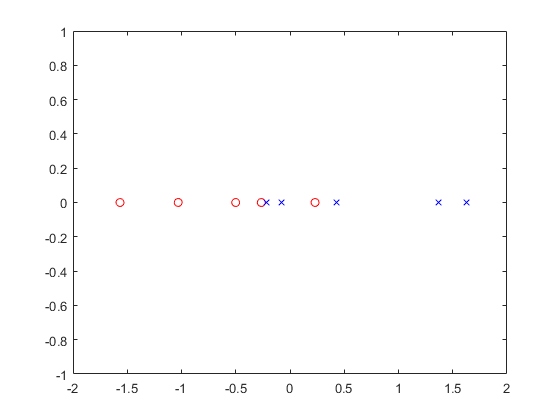
\includegraphics[scale=1.2]{TQ2_e.png}
\caption{Projection of data onto the principal component}
\end{center}
\end{figure}

\newpage

\section{Programming Questions}
\subsection{Dimensionality Reduction via PCA}

Visualization of PCA:

\begin{figure}[h!]
\begin{center}
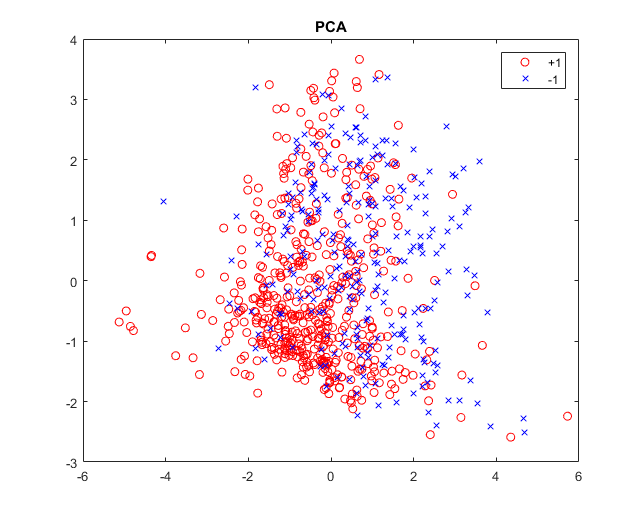
\includegraphics[scale=1.1]{PCA.png}
\caption{Visualization of PCA}
\end{center}
\end{figure}


\newpage
\subsection{Eigenfaces}

\subsubsection{Value of k}
The value of $k$ was found to be $37$.
\subsubsection{Visualization of primary principle component}
\begin{center}

\begin{figure}[h!]
\includegraphics[scale=1.0]{Eigenfaces1.png}
\caption{PCA visualization}
\end{figure}

\end{center}
\newpage
\subsubsection{Visualization of the reconstruction of the first person}
The top row is the visualization with non standardized data while the bottom row is the visualization with standardized data.
\begin{figure}[h!]
\begin{center}
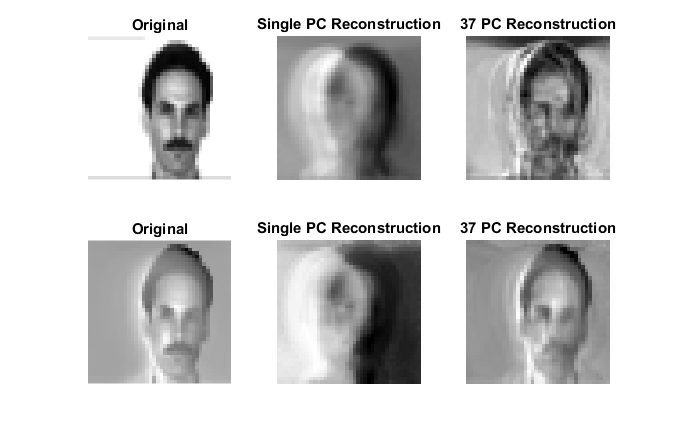
\includegraphics[scale=1.0]{Eigenfaces2.png}
\caption{Visualization of the reconstruction of the first person}
\end{center}
\end{figure}
\end{document}


